\documentclass[12pt, letterpaper]{article}
\usepackage[utf8]{inputenc}
\usepackage{amsmath}
\usepackage[titletoc, title]{appendix}
\usepackage{booktabs}
\usepackage{parskip}

\usepackage{graphicx}
\graphicspath{{../images/}}

\usepackage{hyperref}
\hypersetup{
    colorlinks=true,
    urlcolor=blue,
    linkcolor=blue,
    citecolor=black,
    filecolor=blue,
}
\urlstyle{same}

\title{Notes to Results}
\author{}
\date{}


\begin{document}
\maketitle

\section{Predictive Performance}

%%%
\begin{figure}[t]
    \centering
    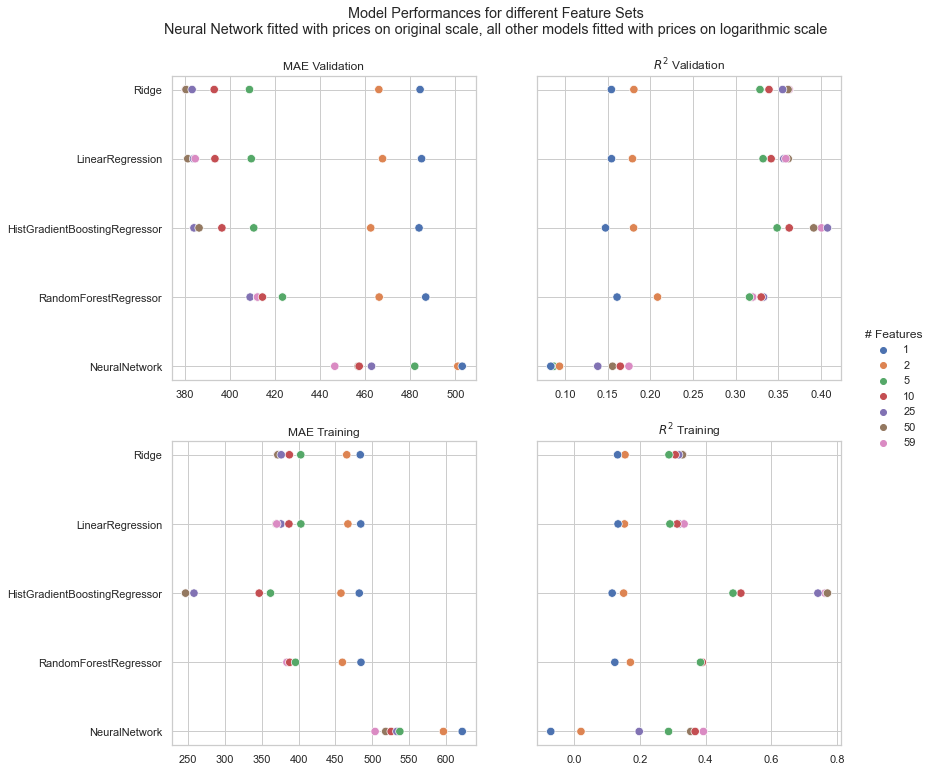
\includegraphics[width=\textwidth]{model_comparison.png}
    \caption{Performance Comparison of Classical Models with Neural Network}
    \label{fig:model-comparison}
\end{figure}
%%%

Figure \ref{fig:model-comparison} shows performance metrics for all fitted models on both the Training Set and the Validation Set.
Whereas we used the Mean Squared Error Loss for \emph{training} the Neural Net due to its convenient differentiability with regards to backpropagation, we focused on the Mean Absolute Error and the $R^2$ value for \emph{evaluating} all regression models.
The MAE measures absolute deviations between true and predicted price and is therefore interpretable on the same scale as the original data.
While the $R^2$ certainly has some inherent flaws, it provides a scale-independent and highly interpretable measure of overall model fit.

The different colors in figure \ref{fig:model-comparison} indicate how many features were selected by the \texttt{RFE} algorithm for this particular fit with $59$ total predictor variables.
Unsurprisingly, one or two features (in case of the \texttt{RFE} the number of bedrooms and the (number of) accomodates) provide too little information to model the task appropriately.
However, including merely $5$ features (in this case adding the $30$ day availability, the indicator variable for the \emph{Frogner} neighbourhood and, notably, the price predictions from the Convolutional Net based on the image data) results in a very competitive performance for most models on the validation set.

The two subplots on the left displaying the MAE tell a very similar story to the subplots on the right that show the $R^2$:
Generally, more features lead to better performance on training and validation set.
In case of the flexible Histogram-based Gradient Boosting algorithm and, to some minor extent, for the Random Forest, a high number of input features lead to \emph{overfitting} such that the performance on the training set is far superior to the values on out-of-sample data.
In contrast, models with few parameters such as Linear Regression or Ridge Regression generalize very well to the validation set with virtually no performance drop.

One exception to this rule is the highly complex Neural Network which appears to perform \emph{better} on out-of-sample data.
This phenomenon can be explained to some extent by the different behaviour of Dropout and Batchnorm during training and inference and was already discussed in the previous chapter.

When comparing the models within each subplot, all classical Machine Learning models perform similarly on the validation data.
This finding emphasizes two aspects:
%%%
\begin{enumerate}
    \item The prediction task does \textbf{not} require overly complex models and linear models perform just fine.
    \item We can expect predictions within a distance of roughly $400$ NOK (40 Euros) on average to the true price.
          Further, a $R^2$ value of around $0.4$ is the best we can hope for.
          These statements hold for fitting on the \emph{entire} training set, section \ref{outliers} reveals how the performance radically improves when excluding some observations.
\end{enumerate}
%%%
In comparison to all \texttt{scikit-learn} models our custom Neural Net appears to underperform.
We have to keep in mind, though, that evaluation on the validation set is overly optimistic for those models whose hyperparameters were tuned on this data during cross validation.
The best simulation to performance on truly unseen data is thus provided by the \emph{test} set that was not used in any step up to this point.

\begin{table}[t]
    \centering
    \begin{tabular}{@{}ccc@{}}
        \toprule
        \multicolumn{1}{l}{} & \multicolumn{1}{l}{MAE} & \multicolumn{1}{l}{\textbf{$R^2$}} \\ \midrule
        Linear Regression    & 404.709                 & 0.298                              \\
        Ridge                & 405.932                 & 0.294                              \\
        Random Forest        & 444.166                 & 0.268                              \\
        HistGradientBoosting & 412.243                 & 0.387                              \\
        Neural Network       & 402.24                  & 0.333                              \\
        Top2 Average         & 404.848                 & 0.296                              \\
        Top3 Average         & 399.315                 & 0.343                              \\
        Top4 Average         & 404.206                 & 0.332                              \\
        Top5 Average         & 408.116                 & 0.27                               \\ \bottomrule
    \end{tabular}
    \caption{Test Set Performance of Classical Machine Learning Models, our custom Neural Network and Ensemble Predictions}
    \label{tab:test-set}
\end{table}

Table \ref{tab:test-set} compares test set metrics for the best performing models on the validation set within each class (i.e. the Neural Net version with all $59$ features and the Random Forest model with only $25$ features were selected).
In addition, we added some simple ensemble models that predict the average estimate from the top $2$, $3$, $4$ or all five models, respectively.

Quite surpringly, the Neural Net shows a significant performance boost on the Test Set and is now very competitive with all other models.
The Random Forest Model generalizes worst and suffers from overfitting given its selected hyperparameter configuration.
Averaging predictions from multiple algorithms indicates promising results:
The Top $3$ Average achieves the lowest out-of-sample Mean Absolute Error of slightly below $400$ NOK.




\section{Understanding and Interpretation}

Interpreting the results of high-dimensional and complex statistical models is notoriously difficult.
This section approaches the challenge from two opposite angles.

First, we reduce the \emph{complexity} by fitting a simple and well-understood Linear Regression Model with the same features that were selected for the best-performing Neural Network and analyze the coefficients.

Second, we reduce the \emph{dimensionality} by leveraging a different Neural Network and visualize the results in two-dimensional space.

\subsection{Feature Importance}

In order to draw conclusions about which features were most important for the Neural Network one could imagine to compute gradients of the single output node with respect to each input node by backpropagating through the entire network.
We chose to analyze the feature importance of an auxiliary Linear Regression model instead to provide some suggestions that could potentially apply to the Neural Network as well.

Therefore we preselected $25$ of the network's input features with the \texttt{RFE} algorithm introduced in the previous chapter and compared the coefficient magnitudes.
As noted before, all predictors were standardized such that a meaningful comparison is feasible.
The results are shown in figure \ref{fig:coefficient-plot} in the Appendix.

It is worth noting that the two most important features based on various different feature selectors of the \texttt{scikit-learn} library were always the number of \emph{bedrooms} and the (number of) \emph{accomodates} in this order, both measuring the apartment's \emph{capacity}.

The coefficient plot, however, is dominated by categorical features:
In agreement with human intuition the \emph{room} type, the \emph{property} type and the \emph{neighbourhood} strongly influence the predicted price.
Unsurprisingly, the property types \emph{entire home} and \emph{entire villa} are connected with high prices, whereas the the room type \emph{shared room} correlates with cheaper apartments.
Notably, the price predictions from the Convolutional Network fitted on the image data indicates a significant positive effect, conditioned on all other selected features.

When analyzing the \emph{marginal} effect of neighbourhood on price by e.g. ordering the neighbourhoods according to their median price, this order is nearly identical to the ranking in figure \ref{fig:coefficient-plot} with \emph{Frogner} at the top and \emph{Grorud} at the bottom.

Interestingly, apartments in the \emph{Sentrum} (central area) have a large positive coefficient in the regression, yet the second to lowest median price.
This finding indicates the presence of \emph{confounders}:
The city center might plausibly be connected to fewer rooms and smaller apartment sizes overall pulling the median price down.
These confounding effects are controlled for in the regression model but not in the naive bivariate analysis.


\subsection{Sensitivity to Outliers} \label{outliers}

% Manually constructed with saved .csv file in tables folder and
% https://www.tablesgenerator.com/latex_tables
\begin{table}[t]
    \centering
    \begin{tabular}{@{}ccc@{}}
        \toprule
        \textbf{Quantile Threshold} & \textbf{MAE} & \textbf{$R^2$} \\ \midrule
        0.0                         & 443.35       & 0.16           \\
        1.0                         & 337.59       & 0.51           \\
        2.5                         & 282.17       & 0.53           \\
        5.0                         & 240.57       & 0.54           \\
        10.0                        & 214.76       & 0.49           \\ \bottomrule
    \end{tabular}
    \caption{Mean Absolute Error and $R^2$ value of the Neural Network on the validation set after removing the highest quantiles of the price distribution from the data set}
    \label{tab:mlp-outliers}
\end{table}

Table \ref{tab:mlp-outliers} shows performance metrics for the Neural Network fitted on a subset of the data in the validation set.
As indicated by the first column the dataset was reduced by successively cutting off observations from the top of the price distribution.
More precisely, the first row refers to the entire data whereas the last row excludes the top $10$\% most expensive apartments.

By omitting just the top $1$\%, the MAE reduces by over $100$ NOK (about $10$ Euros) and the $R^2$ rapidly jumps to over $0.5$.
This sensitivity to outliers in the price distribution is \textbf{not} solved by log-transforming the price, all classical models from the previous chapter suffer from the same effect.

Clearly, the Neural Network lacks the ability to capture the entire price range accurately.
There are two possible explanations for this phenomenon:
%%%
\begin{enumerate}
    \item The model is flawed.
    \item The model is faced with a nearly impossible task.
\end{enumerate}
%%%
In order to discriminate the observations with the highest prices from all other listings, the corresponding feature combinations must be separable in the full $59$-dimensional feature space.
Since this high-dimensional space cannot be visualized, we approximate it with an two-dimensional \emph{embedding} or \emph{latent space}.
If the price outliers are clearly separated from the rest in this embedded space, the network is faced with a feasible task.
If, however, the outliers are located in the \emph{middle} of the latent distribution, there is little hope to discriminate the most expensive apartments from any of their potentially much lower priced embedded neighbours.

Modern Machine Learning methods provide a large toolbox for low-dimensional embeddings.
Since the project is mainly focused on Deep Learning we decided to use a \emph{Variatonal Autoencoder} \cite{kingma2014}.
In contrast to deterministic Autoencoders the VAE contains an additional loss term apart from the usual reconstruction loss that pulls the encoded latent space distribution towards an isotropic multivariate Gaussian distribution.
For this reason, latent space visualizations of the VAE appear to be more spread out and output classes (that are not used for training the VAE) tend to be easier to identify.

%%%
\begin{figure}[t]
    \centering
    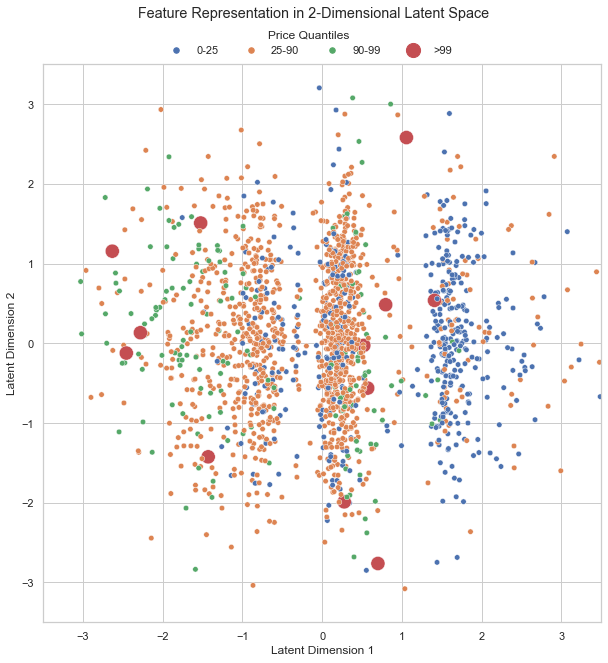
\includegraphics[width=0.8\textwidth]{latent_representation.png}
    \caption{Feature Representation in a two-dimensional latent space embedding}
    \label{fig:latent-representation}
\end{figure}
%%%

Figure \ref{fig:latent-representation} visualizes the two-dimensional feature embedding.
Already a \emph{single} dimension seems so be sufficient for a general understanding of price segments.
While some of the most expensive apartments are located on the far left, surrounded by highly-priced neighbours, the other half shares a similar feature representation to \emph{medium to low} priced listings.
Hence, the network likely maps this second half to comparably low price predictions resulting in large residuals with a high influence on the MAE and the $R^2$ value.

Assuming that the two-dimensional picture appropriately reflects the situation in the full feature space there are two possible explanations for this lack of separability:
%%%
\begin{enumerate}
    \item The collected data is simply not rich or expressive enough to capture all factors that contribute to very high prices.
    \item Some apartments are listed at a price that does not represent their true value.
\end{enumerate}
%%%

In the latter case it can be argued that the entire task of predicting Airbnb prices is flawed in the first place:
In order to draw connections from features to outputs the process implicitly assumes observations whose listed price can be justified and explained by characteristics of the joint feature distribution.

Moreover, discriminating between these two options is nontrivial.
One idea is to use features like availability or the number of reviews to approximate demand and classify price outliers with low demand as overpriced.
However, it is entirely possible that an extremely expensive observation with very low demand is listed according to its true value, yet nobody is willing to pay such a high amount for an accomodation, regardless of its quality.
As a consequence, a blind removal of such outliers is difficult to justify when obeying correct statistical methodology.


\begin{appendices}
    \section{}
    \subsection{Feature Importance}

    %%%
    \begin{figure}[ht]
        \centering
        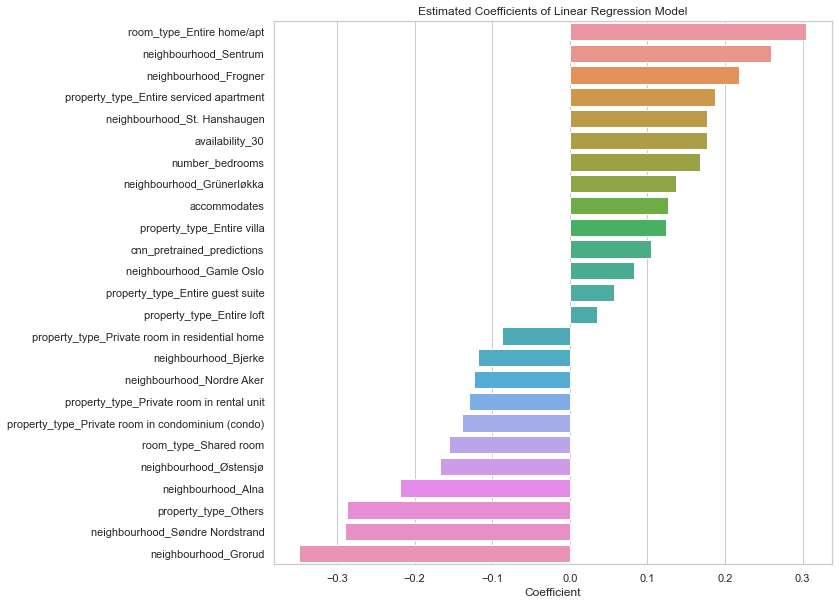
\includegraphics[width=\textwidth]{coefficient_plot.png}
        \caption{Estimated coefficients of a Linear Regression model for $25$ preselected features}
        \label{fig:coefficient-plot}
    \end{figure}
    %%%
\end{appendices}

\bibliography{../bib}
\bibliographystyle{apalike}

\end{document}